% ============================================================
% Capstone Proposal - Starlink-Primary Resilient Gateway Reference Lab
% Print version (short: ~2 pages, one diagram). Compile: pdflatex x2
% Edit the two macros below (name, date) before printing.
% ============================================================
\documentclass[11pt,letterpaper]{article}

\usepackage[T1]{fontenc}
\usepackage[utf8]{inputenc}
\usepackage[margin=1in,top=0.75in,bottom=0.75in]{geometry}
\usepackage[scaled=.96]{helvet}
\renewcommand{\familydefault}{\sfdefault}
\usepackage{microtype}
\usepackage{xcolor}
\usepackage{graphicx}
\usepackage{titlesec}
\usepackage{enumitem}
\usepackage{fancyhdr}
\usepackage{lastpage}
\PassOptionsToPackage{hyphens}{url}
\usepackage[colorlinks=true, urlcolor=PrimaryBlue, linkcolor=PrimaryBlue]{hyperref}

% ---- Blue palette ------------------------------------------
\definecolor{AccentBlue}{HTML}{3A83C2}  % medium blue: rules, bullets, box
\definecolor{PrimaryBlue}{HTML}{1B5A8F} % dark blue: headings, links, keyphrases
\definecolor{Slate}{HTML}{273140}       % near-black slate: title
\definecolor{Muted}{HTML}{5A6470}       % gray: bylines, captions

% ---- Fill these in -----------------------------------------
\newcommand{\preparedby}{Havi Arji}
\newcommand{\proposaldate}{July 2026}

% ---- Layout ------------------------------------------------
\setlength{\parindent}{0pt}
\setlength{\parskip}{3.5pt}

\setcounter{secnumdepth}{0}
\titleformat{\section}
  {\large\bfseries\color{PrimaryBlue}}{}{0pt}{}
  [{\vspace{-2pt}\color{AccentBlue}\titlerule[1.1pt]}]
\titlespacing*{\section}{0pt}{8pt}{4pt}

\setlist[itemize]{leftmargin=1.2em, itemsep=2pt, topsep=2pt,
  label=\textcolor{AccentBlue}{\textbullet}}
\setlist[enumerate]{leftmargin=1.4em, itemsep=2pt, topsep=2pt,
  font=\bfseries\color{PrimaryBlue}}

\pagestyle{fancy}
\fancyhf{}
\renewcommand{\headrulewidth}{0pt}
\fancyfoot[L]{\footnotesize\color{Muted} Starlink-Primary Gateway Reference Lab --- Capstone Proposal}
\fancyfoot[R]{\footnotesize\color{Muted} Page \thepage\ of \pageref{LastPage}}

\newcommand{\keyphrase}[1]{\textbf{\textcolor{PrimaryBlue}{#1}}}

\begin{document}

% ---- Title block -------------------------------------------
{\color{AccentBlue}\rule{\linewidth}{4pt}}

\vspace{8pt}
{\LARGE\bfseries\color{Slate} Starlink-Primary Resilient Gateway\\[2pt] Reference Lab\par}

\vspace{4pt}
{\large\bfseries\color{PrimaryBlue} Internship Capstone Proposal\par}

\vspace{3pt}
{\small\color{Muted} Prepared by \preparedby\ \ \textbullet\ \ Digi International\ \ \textbullet\ \ \proposaldate\par}

% ---- Executive summary -------------------------------------
\section{Executive summary}

\setlength{\fboxsep}{10pt}\setlength{\fboxrule}{0.8pt}%
\noindent\fcolorbox{AccentBlue}{AccentBlue!6}{%
\begin{minipage}{\dimexpr\linewidth-2\fboxsep-2\fboxrule\relax}
Before I finish my internship, I want to build a \keyphrase{repeatable reference lab}: \keyphrase{Starlink as the primary WAN, backed by Digi 5G, managed as code through Digi Remote Manager}, with an embedded ConnectCore (Yocto) site sensor and a \keyphrase{measured comparison of native SureLink failover vs.\ Digi WAN Bonding} --- validated with real fault injection, and demoed from an iPad as a \keyphrase{live, tappable diagram of the lab}.

\vspace{3pt}
\textit{\color{PrimaryBlue}Two focused weeks. I'd like to leave Digi with a reusable asset, not just a nice internship.}
\end{minipage}}

% ---- Why worth authorizing ---------------------------------
\section{Why it's worth authorizing}

\begin{itemize}
  \item \textbf{A sellable reference architecture} --- ``Starlink primary + Digi 5G + Opengear out-of-band'' --- that pre-sales and enablement can demo on demand.
  \item \textbf{Quantitative interoperability data} --- native failover vs.\ WAN Bonding, by firmware, carrier, IPv4/IPv6 and MTU.
  \item \textbf{Concrete findings for Product/Docs} --- a register of a dozen documentation gaps and contradictions I'll close against real tenants and hand back with recommended owners.
\end{itemize}

% ---- Fit + demo (one diagram) ------------------------------
\section{Where it fits Digi's story --- and the demo you can touch}

The closest of Digi's industry solution pages is \keyphrase{Energy \& Utilities}\footnote{\url{https://www.digi.com/solutions/by-industry/energy-and-utilities}} --- Digi IX routers at remote sites, ``Utility Network Failover Management,'' Digi Remote Manager at the center, plus XBee and ConnectCore. Digi's own WAN Bonding + Starlink post\footnote{\url{https://www.digi.com/blog/post/digi-wan-bonding-starlink-ultra-fast-internet}} names these use cases but stops at the concept level. \keyphrase{This lab makes it real and measurable} --- and it demos from an iPad: a live, tappable diagram where you tap a device to see its status (which WAN is carrying traffic, signal, last failover) straight from the DRM API, and watch Starlink fail over to 5G in near-real time.

\begin{center}
  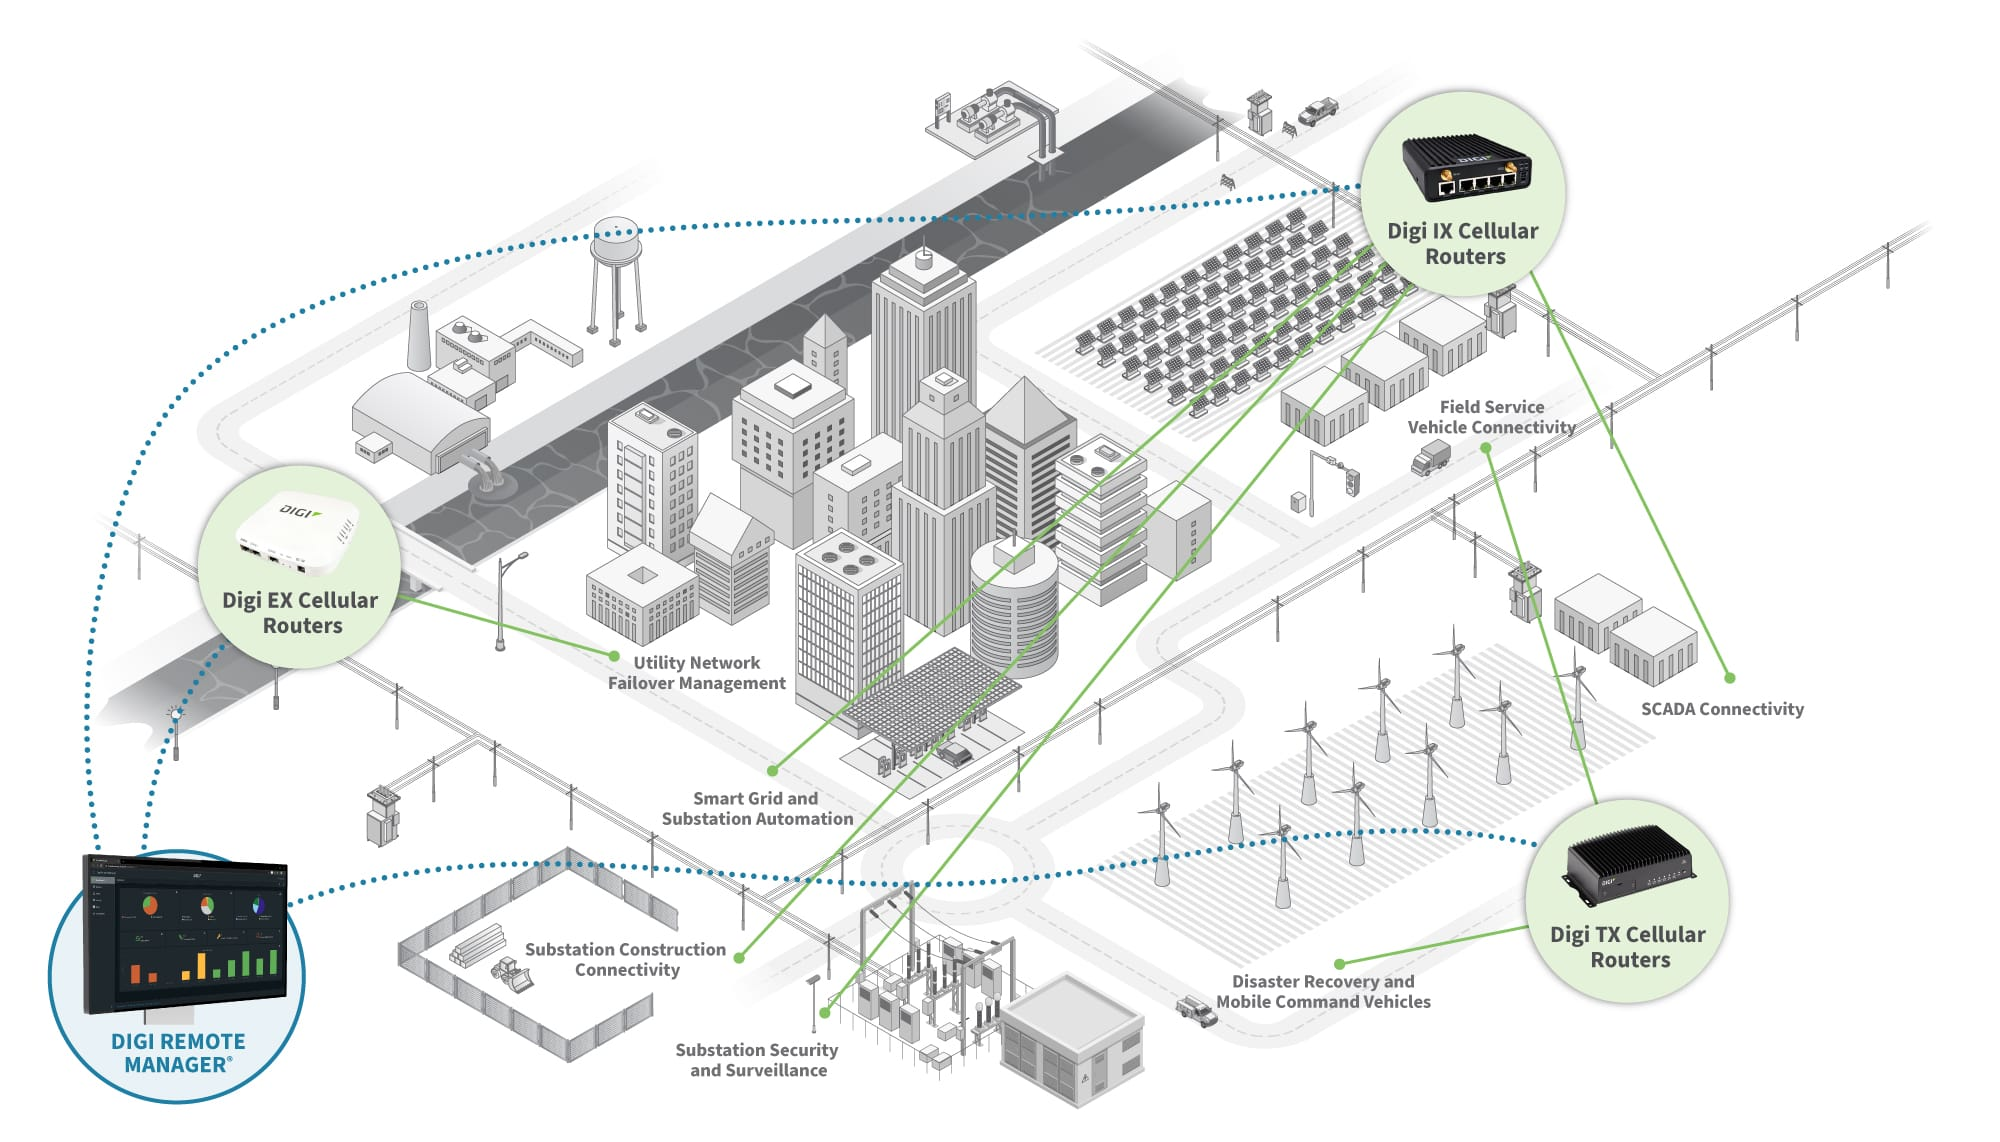
\includegraphics[width=0.52\linewidth]{assets/digi-energy-utilities-diagram.jpg}\\[3pt]
  {\footnotesize\color{Muted} Digi Energy \& Utilities managed-solutions diagram --- the architecture this lab embodies.\\ Source: \url{https://www.digi.com/solutions/by-industry/energy-and-utilities}}
\end{center}

% ---- Scope -------------------------------------------------
\section{Scope: honest about two weeks}

I won't pretend a 10-week program fits in two, so it's built in concentric rings:

\begin{itemize}
  \item \textbf{\textcolor{PrimaryBlue}{Ring 0 --- the 2-week commitment:}} one site end to end (Starlink + 5G, DRM-as-code, BGP/IPv6, \textit{measured} SureLink failover); the embedded ConnectCore sensor working (custom Yocto image + agent + offline buffer that loses nothing on a link cut; \textit{secure boot deferred to Ring 2}); XBee telemetry + a Digi Container; one-command site-clone automation; a native-vs-WAN-Bonding A/B; the iPad app for site~1; and a recorded 12-minute demo.
  \item \textbf{\textcolor{PrimaryBlue}{Ring 1 --- as hardware arrives:}} sites 2--3 via the same automation, the Opengear\slash Lighthouse out-of-band plane, and the app's three-site view.
  \item \textbf{\textcolor{PrimaryBlue}{Ring 2 --- the full program:}} three-site rotation, a 30-rep statistical campaign, TrustFence secure boot, secure OTA, and the full interoperability matrix.
\end{itemize}

\textbf{On Opengear:} the entire critical path runs on Digi equipment, so Opengear's lead time (Ring~1) can't block the capstone.

% ---- The ask -----------------------------------------------
\section{What I'm asking you to authorize}

For the 2-week sprint, one of each is enough (more only to build sites 2--3):

\begin{itemize}
  \item \textbf{Hardware:} 1$\times$ IX40-05 (+ starter kit + DIN mount), 1$\times$ ConnectCore \texttt{CC-WMP255-KIT}, 1$\times$ XBee Hive + XBee 3 Zigbee kit.
  \item \textbf{Licenses/services:} DRM Premier + Digi Containers, a WAN Bonding Tier-3 trial + a small bonding VPS, and confirmation our tenant carries Push Monitor and ConnectCore Cloud Services entitlements.
  \item \textbf{Connectivity:} one Starlink Priority plan and one 5G SIM. \quad\textbf{Already have:} Proxmox, SIEM, RADIUS.
  \item \textbf{In parallel (can arrive later):} Opengear OM1304 + Lighthouse Enhance and second/third units --- for Rings 1--2.
\end{itemize}

Nothing gets purchased before its verification gate closes --- in particular, \keyphrase{no SFP+ (the IX40 is SFP-only)}.

% ---- What I need -------------------------------------------
\section{What I need from you}

A \textbf{yes} on the sprint scope and the equipment above, \textbf{sign-off} on objectives and publication rules, and \textbf{15 minutes} on day zero to align on success criteria. I already run the adjacent pieces (Lighthouse, Proxmox, SIEM, RADIUS), so the scaffolding exists. If any assumption slips (hardware lead time, a plan's IPv6 behavior), I'll adjust scope transparently rather than overclaim.

\vspace{5pt}
\textit{\color{PrimaryBlue}Thank you --- I think this is the most useful two weeks I could spend here.}

\end{document}
